\documentclass[main.tex]{subfiles}

\begin{document}

\section{Summary}
\label{sec:summary}
   
This report was developed due to the curricular course RCOM(Computer Network) and it serves the purpose of concluding the first project of this course.
The project was finished successfully by implementing all the required functionalities, passing all the tests and building a fully working application while adding options that were not required specified further in the report.

% This section needs a lot of work.
\subsection{Introduction}
\label{subsec:intro}

This project’s goal is to transfer data from one computer to the other through a serial port using a protocol developed by us which includes reading, writing and data analysis functions.
We did all this based on the script provided to us.
In here you will be able to find all the functions used by us to achieve the goal and and explanation of almost everything using this structure:

Architecture - functional blocks and interfaces used
Code Structure - demonstration of the API’s, main data structuring, functions and how they relate to the architecture
Main use cases - sequence of functions with the help of diagrams created by us
Linking layer protocol - identification of the main functional aspects, description of those aspects implementation strategy with code samples
Application protocol - identification of the main functional aspects, description of those aspects implementation strategy with code samples
Validation - description of the tests used with data to back up the test results
LL protocol efficiency - stats that measure the protocol’s practical efficiency and also the theoretical efficiency used as comparison
Conclusion - reflection on the learning objectives achieved and also an overall view of the information detailed on the previous sections.

\subsection{Concepts}
\label{subsec:concepts}

$AL$ - Application Layer\\
$R$ - Receiver\\
$T$ - Transmitter\\
$LL$ - Link Layer\\

\section{Architecture}
\label{sec:arch}

We will now traverse \textit{bottom-up} the program's architectural aspects, including the internal and auxiliary functions of each layer, their interfaces and the primary data structures used. We will also discuss some parallel features, such as terminal setup, program options, signal handlers, execution timing and forced error introduction.

\subsection{String}
\label{subsec:string}

Given that the byte arrays used throughout the program are \emph{not} \nullp-terminated strings --- but rather variable length and dynamically allocated --- they must be \textit{accompanied} by their size anytime they are passed between functions. The \struct{string} structure is a simple wrapper around a \struct{char*} and a \struct{size_t}.

\subsection{Link Layer}
\label{subsec:llarch}

The link layer's core contains one fundamental, yet simple data structure: \struct{frame}. It holds information both for the frame's header ($A$ and $C$ fields) and the frame's data field.

\subsubsection{Functions}
\label{subsubsec:funcllarch}

The core has the following functions:

\begin{itemize}[noitemsep,rightmargin=3em]
	\item Byte stuffing and destuffing: \function{stuffData}, \function{destuffData}, \function{destuffText}
	\item Convert a \struct{frame} to a \struct{string} and write it to the device: \function{buildText}, \function{writeFrame}
	\item Read text from the device and convert it to a \struct{frame}:
	\function{readText}, \function{readFrame}
\end{itemize}

On top of these, we have simple utility functions used by the interface:

\begin{itemize}[noitemsep,rightmargin=3em]
	\item Inquire frames: \function{is*frame} --- \function{isIframe}, \function{isSETframe}, \textellipsis
	\item Write frames: \function{write*frame} --- \function{writeIframe}, \function{writeSETframe}, \textellipsis
\end{itemize}

And the interface follows the specification:

\begin{itemize}[noitemsep,rightmargin=3em]
	\item Establish a connection through an open device: \function{llopen}
	\item Terminate a connection through an open device: \function{llclose}
	\item Write a message (frame): \function{llwrite}
	\item Read a message (frame): \function{llread}
\end{itemize}

It should be noted that \function{llopen} and \function{llclose} \emph{do not} open or close the device, nor do they modify any terminal settings.

\subsection{App Layer}
\label{subsec:alarch}

The app-layer makes public three data structures: \struct{tlv}, \struct{control_packet} and \struct{data_packet}. The control packet holds a sequence of \struct{tlv}, which are type/value pairs as described in the introduction. The data packet holds information for both the packet's header field and data field.

\subsubsection{Functions}
\label{subsubsec:funcalarch}

The app-layer core has the following internal functions:

\begin{itemize}[noitemsep,rightmargin=3em]
	\item Convert integers and strings to \struct{tlv}s: \function{build_tlv_str}, \function{build_tlv_uint}
	\item Convert a generic array of \struct{tlv}s to a \struct{control_packet}: \function{build_control_packet}
	\item Convert a \struct{string} to a \struct{data_packet}: \function{build_data_packet}
	\item Extract any \struct{tlv} value from a \struct{control_packet}: \function{get_tlv}
	\item Inquire packets: \function{isDATApacket}, \function{isSTARTpacket}, \function{isENDpacket}
\end{itemize}

The interface provided to the application user includes:

\begin{itemize}[noitemsep,rightmargin=3em]
	\item Send control and data packets using llwrite and llread: \function{send_data_packet}, \function{send_start_packet}, \function{send_end_packet}
	\item Receive (any) packet using llwrite and llread:
	\function{receive_packet}
	\item Extract filename and filesize from a \struct{control_packet}: \function{get_tlv_filesize}, \function{get_tlv_filename}
\end{itemize}

\subsection{Parallel features}
\label{subsec:parallelarch}

\begin{itemize}[noitemsep,rightmargin=3em]
	\item Open chosen device and set new terminal settings: \function{setup_link_layer}
	\item Close chosen device and set old terminal settings: \function{reset_link_layer}
	\item Alarm utilities for write timeouts: \function{set_alarm}, \function{unset_alarm}, \function{was_alarmed}
	\item Execution timing: \function{begin_timing}, \function{end_timing}
	\item Compute and print statistics about error probabilities, communication speed and efficiency: \function{print_stats}
	\item Introduce flip bits in read frames: \function{introduceErrors}
\end{itemize}

\section{Use cases and control flow}
\label{sec:usecases}

\subsubsection{Top level}

Setup in function \function{main} includes parsing and validating program options --- \function{parse_args} ---, setting up signal handlers --- \function{set_signal_handlers} --- testing the system's alarms --- \function{test_alarm} --- and adjusting the terminal configuration (namely noncanonical mode) --- \function{setup_link_layer}. This is the same for $R$ and for $T$.

In function \function{send_file}, called by $T$, the selected file is opened, its size is calculated and it is then read into a single \emph{buffer} and closed. The \emph{buffer} is then split into multiple \emph{packets} with length \var{packetsize} --- each stored in a \struct{string} --- and then freed. These packets are then sent to $R$ in the communications phase, each in its own data packet --- see \autoref{fig:al-transmitter}.

Function \function{receive_file}, called by $R$, enters the communications phase immediately --- see \autoref{fig:al-receiver}. Once the transmission is completed it has received a filename and several packet strings. The output file is created with that filename, the packets are written successively, and then it is closed.

Neither of these functions deal with any $AL$ errors. At the end of \function{main}, the terminal settings are reset with \function{reset_link_layer}.

Simplified sequence diagrams for functions \function{llread} and \function{llwrite} can be found in \autoref{fig:llread} and \autoref{fig:llwrite} respectively.

\begin{figure}[ph]
\caption{Sequence diagrams for some important functions\label{fig:seqdiagrams}}
	
\begin{minipage}{0.5\textwidth}
	\centering
	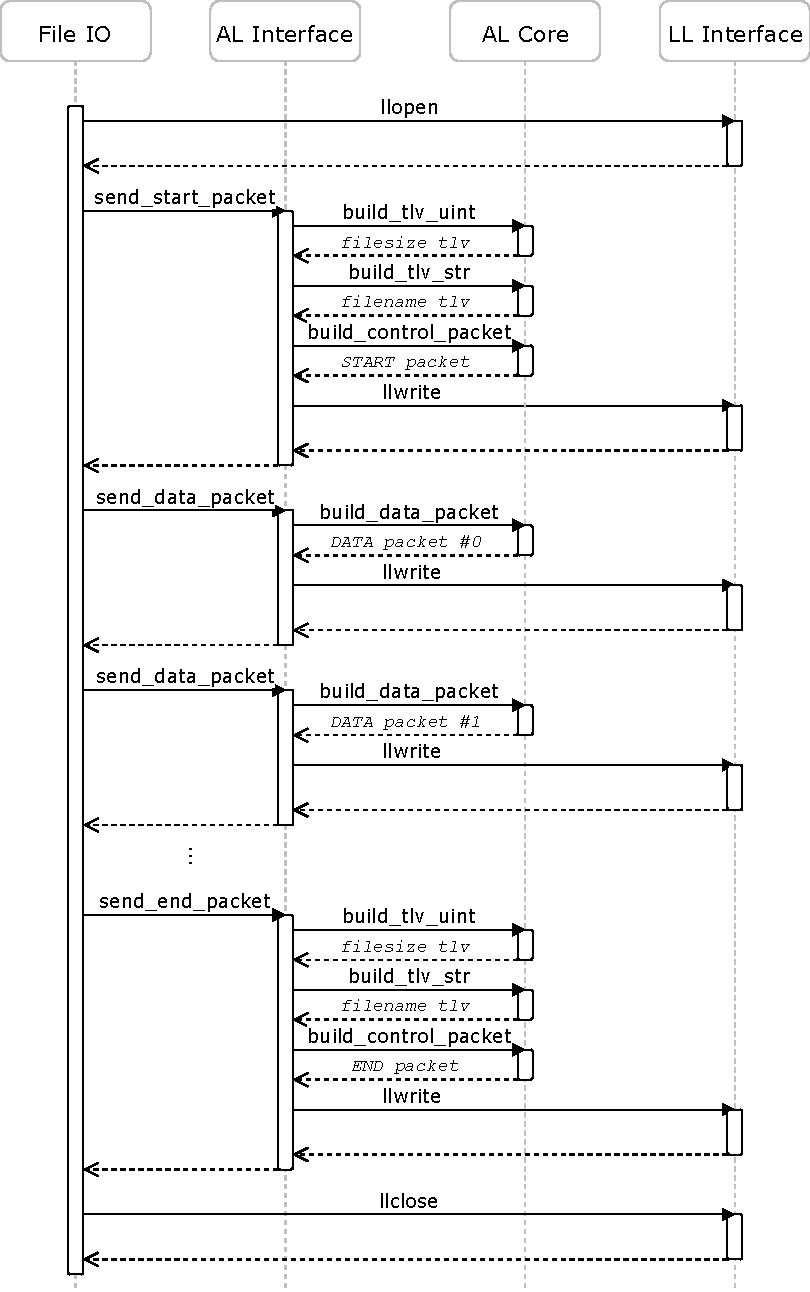
\includegraphics[scale=0.45]{rcom-al-transmitter.pdf}
	\subcaption{File communications as seen through the app layer (part of function \function{send_file})\label{fig:al-transmitter}}
\end{minipage}
\begin{minipage}{0.5\textwidth}
	\centering
	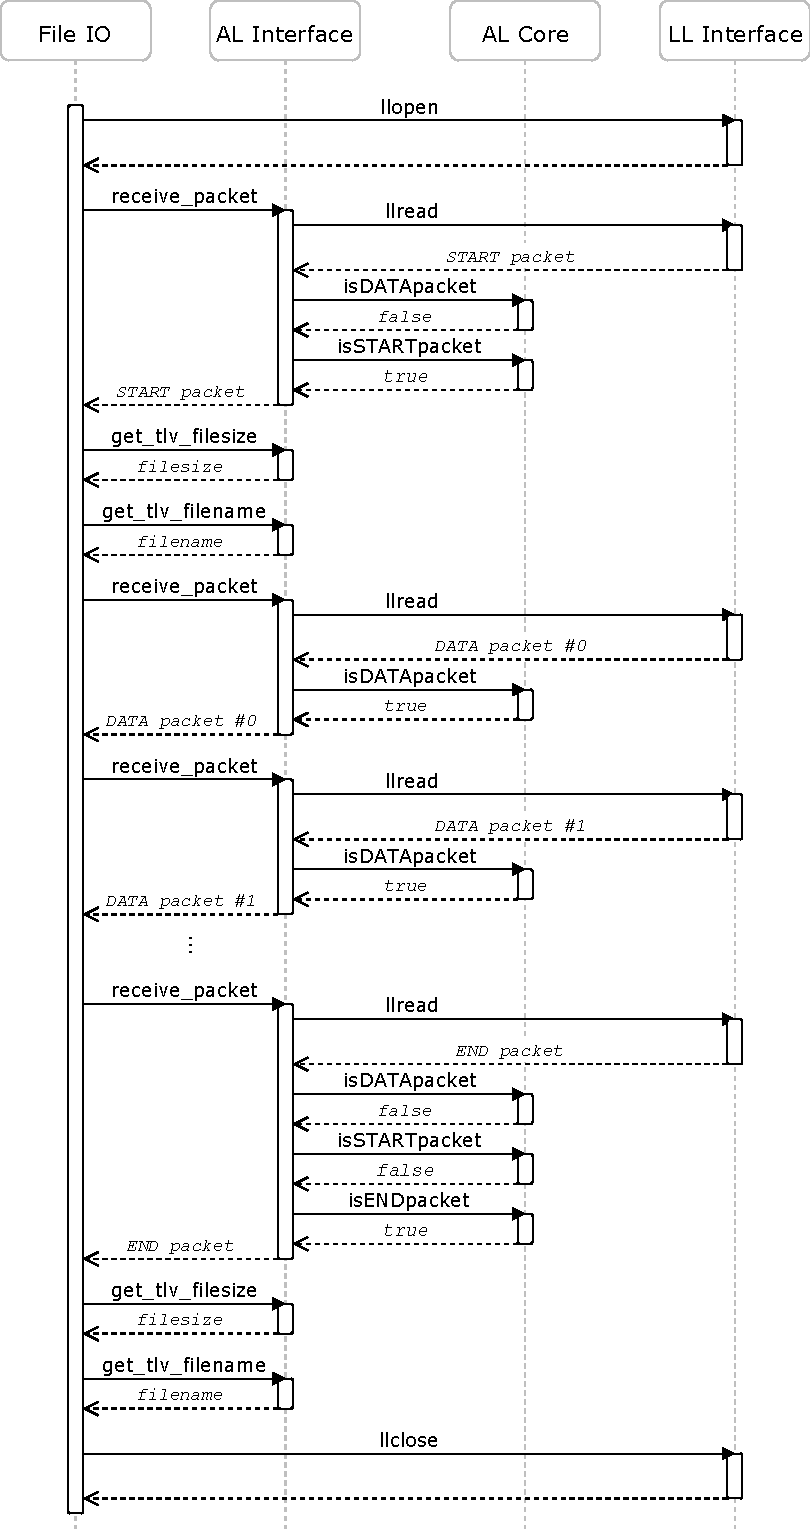
\includegraphics[scale=0.45]{rcom-al-receiver.pdf}
	\subcaption{File communications as seen through the app layer (part of function \function{receive_file})\label{fig:al-receiver}}
\end{minipage}
\begin{minipage}{0.5\textwidth}
	\centering
	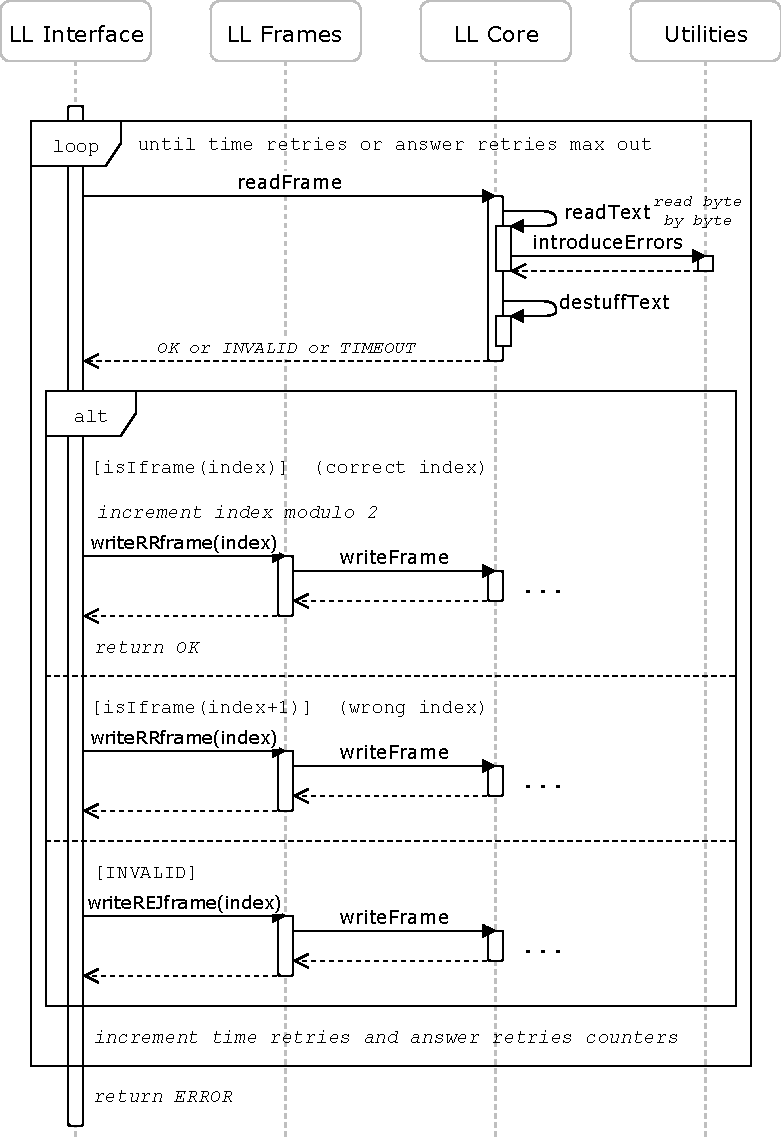
\includegraphics[scale=0.45]{rcom-llread.pdf}
	\subcaption{Function \function{llread}\label{fig:llread}}
\end{minipage}
\begin{minipage}{0.5\textwidth}
	\centering
	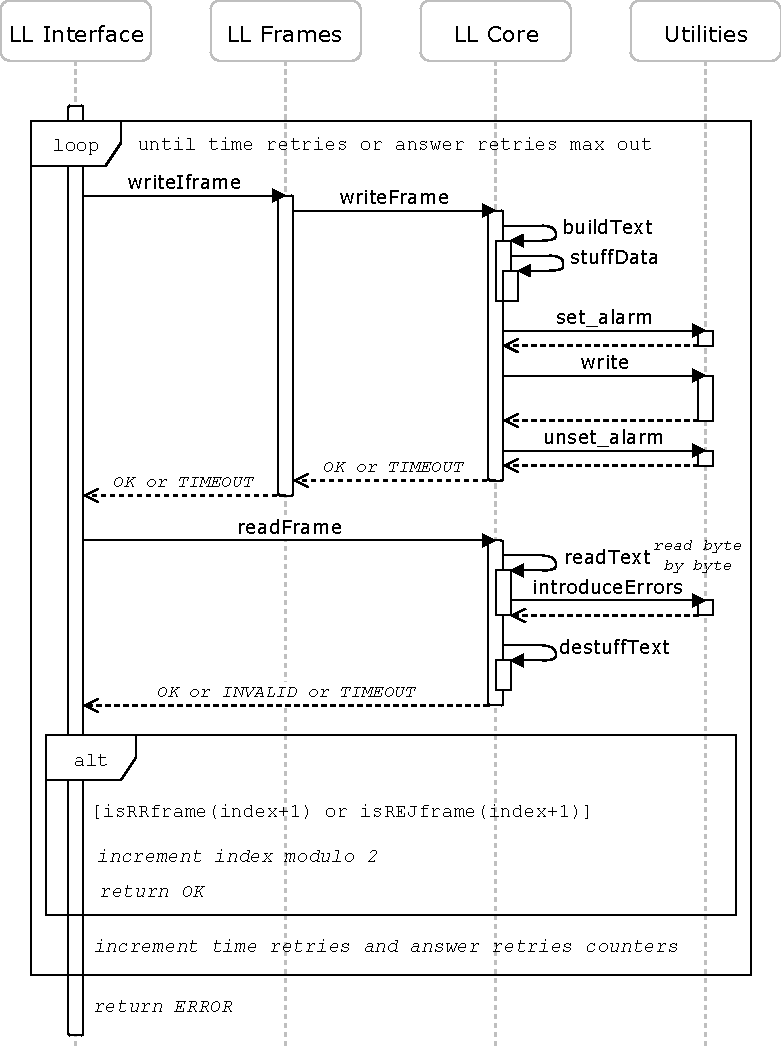
\includegraphics[scale=0.45]{rcom-llwrite.pdf}
	\subcaption{Function \function{llwrite}\label{fig:llwrite}}
\end{minipage}
\end{figure}

\section{Link Layer Protocol}
\label{sec:llprotocol}

\begin{wrapfigure}[40]{r}[1cm]{0.41\textwidth}
\begin{lstlisting}[style=rcom]
static int readText(int fd, string* textp) {
	string text;
	
	text.len = 0;
	text.s = malloc(8 * sizeof(char));
	
	size_t reserved = 8;
	FrameReadState state = READ_PRE_FRAME;
	int timed = 0;
	
	while (state != READ_END_FLAG) {
		char readbuf[2];
		ssize_t s = read(fd, readbuf, 1);
		char c = readbuf[0];
		
		// [...] Errors and text.s realloc

		switch (state) {
		case READ_PRE_FRAME:
			if (c == FRAME_FLAG) {
				state = READ_START_FLAG;
				text.s[text.len++] = FRAME_FLAG;
			}
			break;
		case READ_START_FLAG:
			if (c != FRAME_FLAG) {
				if (FRAME_VALID_A(c)) {
					state = READ_WITHIN_FRAME;
					text.s[text.len++] = c;
				} else {
					state = READ_PRE_FRAME;
					text.len = 0;
				}
			}
			break;
		case READ_WITHIN_FRAME:
			if (c == FRAME_FLAG) {
				state = READ_END_FLAG;
				text.s[text.len++] = FRAME_FLAG;
			} else {
				text.s[text.len++] = c;
			}
			break;
		default:
			break;
		}
	}

	text.s[text.len] = '\0';
	
	introduceErrors(text);
	
	*textp = text;
	return 0;
}



int writeFrame(int fd, frame f) {
	string text;
	buildText(f, &text);
	
	set_alarm();
	errno = 0;
	ssize_t s = write(fd, text.s, text.len);
	
	int err = errno;
	bool b = was_alarmed();
	unset_alarm();
	
	free(text.s);
	
	if (b || err == EINTR) {
		// [...] Report error
		return FRAME_WRITE_TIMEOUT;
	} else {
		return FRAME_WRITE_OK;
	}
}
\end{lstlisting}
\end{wrapfigure}

In the $LL$ protocol we recognize these requirements:

\begin{enumerate}[label=(\alph*),noitemsep,rightmargin=3em]
	\item Canonical, state machine based reading loop of variable length byte arrays;
	\item Timeout in long reads and writes;
	\item Conversions between byte arrays and a generic frame data structure;
	\item Stuffing and destuffing byte arrays, representing valid or invalid generic frames;
	\item Error detection and reporting in read frames;
	\item Probability based error introduction in read frames;
	\item Identification and writing of protocol-defined frames.
\end{enumerate}

Our $LL$ implementation consists of four units: \emph{core}, \emph{errors}, \emph{frames} and \emph{interface}.

\paragraph{Core} The lowest unit of the entire program, it handles the first five requirements. Internally, both in reading and writing. It exposes only \function{writeFrame} and \function{readFrame}, which have \struct{frame} arguments. Function \function{writeFrame} calls \function{buildText} to transform the given \struct{frame} into a string, which is \textit{stuffed} by \function{stuffData} before being written. Function \function{readFrame} calls \function{readText}, the canonical read loop, and destuffs the string read with \function{destuffText}, while validating it and reporting on any detected errors.

This unit supports the entire $LL$ by providing a generic read/write facility for frames of any kind --- supporting all valid frame headers and all frame lengths --- by handling only byte stuffing, error detection, and reading/writing timeouts.

\paragraph{Errors} A simple unit whose purpose is to intentionally introduce errors (bit flips), with a certain probability, in both the header and data fields of frames read at the end of function \function{readText}.

\paragraph{Frames} For each frame in the specification --- \fI{}, \fSET{}, \fDISC{}, \fUA{}, \fRR{}, and \fREJ{} --- this unit exposes a function which identifies it, \function{is*frame}, and another which writes it to a given file, \function{write*frame}.

\paragraph{Interface} Includes specified functions \function{llopen}, \function{llwrite}, \function{llread} and \function{llclose}. These functions use only the facilities provided by the \emph{frames} unit. \function{llopen} is used to establish a connection between $R$ and $T$ by ensuring both ends are in sync; \function{llclose} is used to end it. These functions have different \textit{versions} for $R$ and $T$. While the connection is active, \function{llread} and \function{llwrite} are used to read and write from the connection respectively.

\section{Application Layer Protocol}

\begin{wrapfigure}[38]{r}[1cm]{0.41\textwidth}
\begin{lstlisting}[style=rcom]
static bool isDATApacket(string packet_str, data_packet* outp) {
	char c = packet_str.s[0];
	
	if (packet_str.len < 5 || packet_str.s == NULL || c != PCONTROL_DATA) {
		// [...] Report result
		return false;
	}
	
	int index = (unsigned char)packet_str.s[1];
	unsigned char l2 = packet_str.s[2];
	unsigned char l1 = packet_str.s[3];
	size_t len = (size_t)l1 + 256 * (size_t)l2;
	
	bool b = len == (packet_str.len - 4);
	
	// [...] Report result
	
	if (b) {
		string data;
		
		data.len = len;
		data.s = malloc((len + 1) * sizeof(char));
		memcpy(data.s, packet_str.s + 4, len + 1);
		
		data_packet out = {index, data};
		
		*outp = out;
		
		if (index != in_packet_index % 256) {
			printf("[APP] Error: Expected DATA packet #%d, got #%d\n",
			in_packet_index % 256, index);
		}
	}
	return b;
}



int receive_packet(int fd, data_packet* datap,
	  control_packet* controlp) {
	int s;
	
	string packet;
	s = llread(fd, &packet);
	if (s != 0) return s;
	
	data_packet data;
	control_packet control;
	
	if (isDATApacket(packet, &data)) {
		++in_packet_index;
		*datap = data;
		
		free(packet.s);
		return PRECEIVE_DATA;
	}
	
	if (isSTARTpacket(packet, &control)) {
		in_packet_index = 0;
		*controlp = control;
		
		free(packet.s);
		return PRECEIVE_START;
	}
	
	if (isENDpacket(packet, &control)) {
		in_packet_index = 0;
		*controlp = control;
		
		free(packet.s);
		return PRECEIVE_END;
	}
	
	printf("[APP] Error: Received BAD packet\n");
	free(packet.s);
	return PRECEIVE_BAD_PACKET;
}
\end{lstlisting}
\end{wrapfigure}

In the $AL$ protocol we recognize these requirements:

\begin{enumerate}[label=(\alph*),noitemsep,rightmargin=3em]
	\item Representation of generic control packets and data packets;
	\item Construction of a control packet from a list of values;
	\item Construction of a data packet from a string;
	\item Identification, parsing and writing of protocol-defined packets;
	\item Extraction of \struct{tlv} values from control packets, namely filesize and filename;
	\item Error detection and reporting of mis-indexed \pDATA{} packets or bad packets.
\end{enumerate}

Our $AL$ implementation, unlike the $LL$ implementation, is not further divided. Each of these requirements is satisfied by a set of specialized functions, and the interface is essentially \function{send_data_packet}, \function{send_start_packet}, \function{send_end_packet} and \function{receive_packet}.

The first function, \function{send_data_packet}, takes a \struct{string}, prepends it with a packet header using \function{build_data_packet}, and writes it using \function{llwrite}. The packet index is kept in an internal counter \var{out_packet_index}. The other functions \function{send_start_packet} and \function{send_end_packet} first build two \struct{tlv} for the filesize and filename using \function{build_tlv_*}, then build the control packet string using \function{build_control_packet}, and finally write it using \function{llwrite}.

The \function{receive_packet} function reads an arbitrary packet using \function{llread}, and then uses \function{isDATApacket}, \function{isSTARTpacket} or \function{isENDpacket} to identify \emph{and} parse said packet. The packet index is also kept in an internal counter \var{in_packet_index}.

\section{Validation}
\label{sec:validation}

Some tests were implemented in order to determine the robustness of the program:
\begin{enumerate}[label=(\alph*),noitemsep,rightmargin=3em]
	\item Send a file without errors
	\item Force errors in the serial port with pins
	\item Force errors in the program with specific functions with a specific probability to generate errors in data field and header field (introduceErrors())
	\item Turn off the connection in the serial port and turn it on later
	\item All the previous attempt of failures together.
\end{enumerate}

The program is robust to this errors and much probably others that we did not anticipate. After every single attempt to make the program fail, the connection continues and the file is sent perfectly.

\begin{figure}[htbp]
\centering
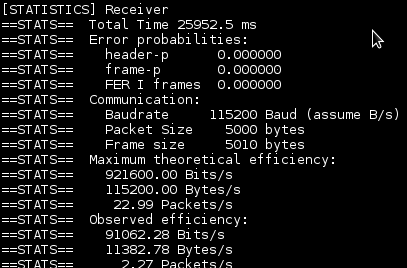
\includegraphics[width=0.45\textwidth]{p=0.png}
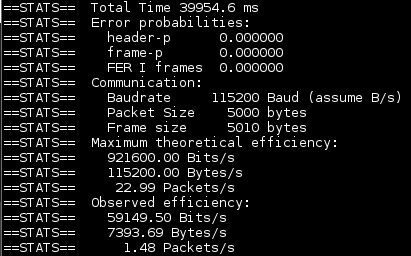
\includegraphics[width=0.45\textwidth]{bcc1-corrupted.png}\\
\medskip
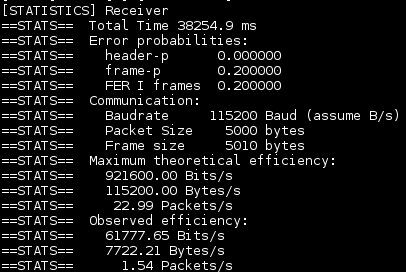
\includegraphics[width=0.45\textwidth]{p=20.png}
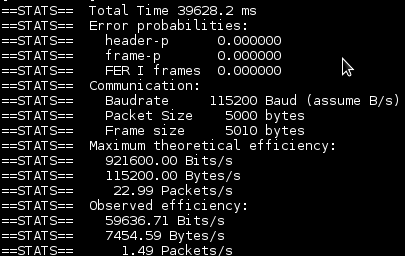
\includegraphics[width=0.45\textwidth]{cut-connection3times.png}
\caption{Output stats for each case}
\label{fig:example}
\end{figure}

\section{Protocol Efficiency}
\label{sec:pefficiency}

To approach this topic we analyze some charts. The first two charts use packets with 5000 bytes of data, baudrate = 115200 and the file has 295412 bytes which corresponds to 59 packets. 

\begin{figure}[htbp]
\begin{minipage}{0.48\textwidth}
\centering
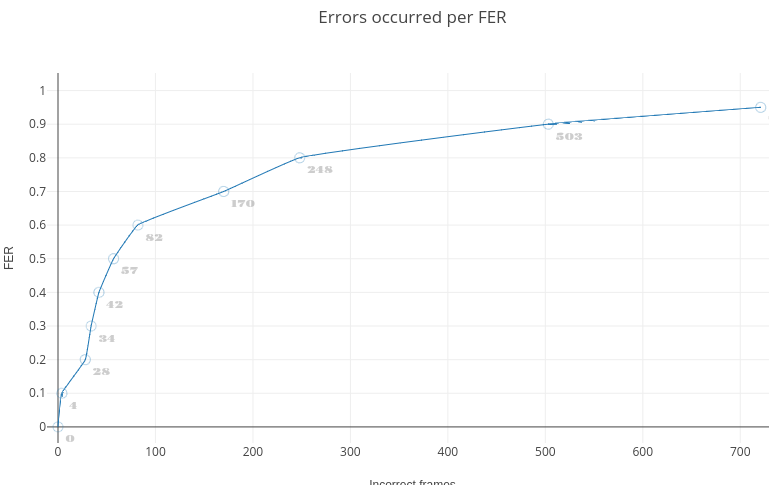
\includegraphics[width=\textwidth]{graph1.png}
\caption{Interpolation for Data 1}
\label{Fig:Data1}
\end{minipage}\hfill
\begin{minipage}{0.48\textwidth}
\centering
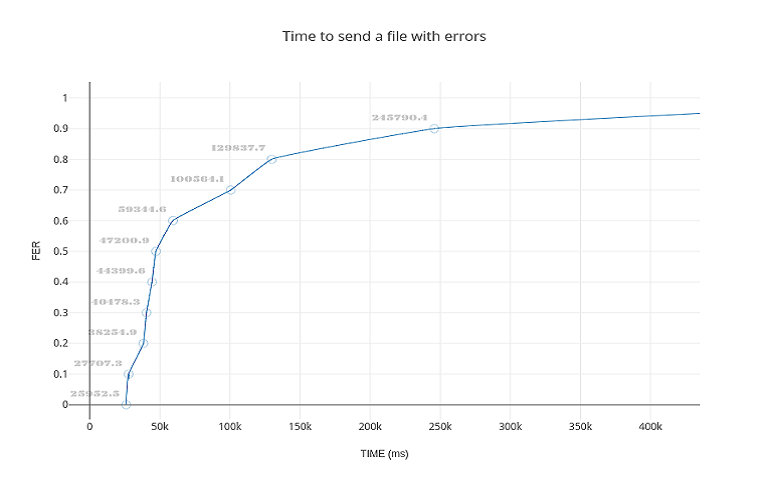
\includegraphics[width=\textwidth]{graph2.png}
\caption{Time to deliver a file with errors}
\label{Fig:Data2}
\end{minipage}
\end{figure}

\section{Conclusion}
\label{sec:conclusion}

We achieved all of the requirements specified on the script building a fully working project. We soaked in all of the concepts of the protocol and we wrote efficient code robust enough to work for multiple frames and to detect multiple failures.

The most challenging part in the development phase was building thellopen() and llclose() functions robust enough so that it detected many errors in the frames headers.

\end{document}
